% TBP-double-Ag100
When adsoped on a (100) silver surface, the molecules arrange in a nice pattern (see figure \ref{fig:two-leg-trans-ag100-motiv}). Although the pattern is dense no problems showed up when designing the molcular models. This is because the last molcules at the perimeter of this island is nicely distinguishable and continuing their regular pattern to the center of the island results in a accurate description of the island.

\begin{figure}[h]
 \centering
 \subfigure[37*37 nm patch of self-assembled molecules adsorped at RT]{
 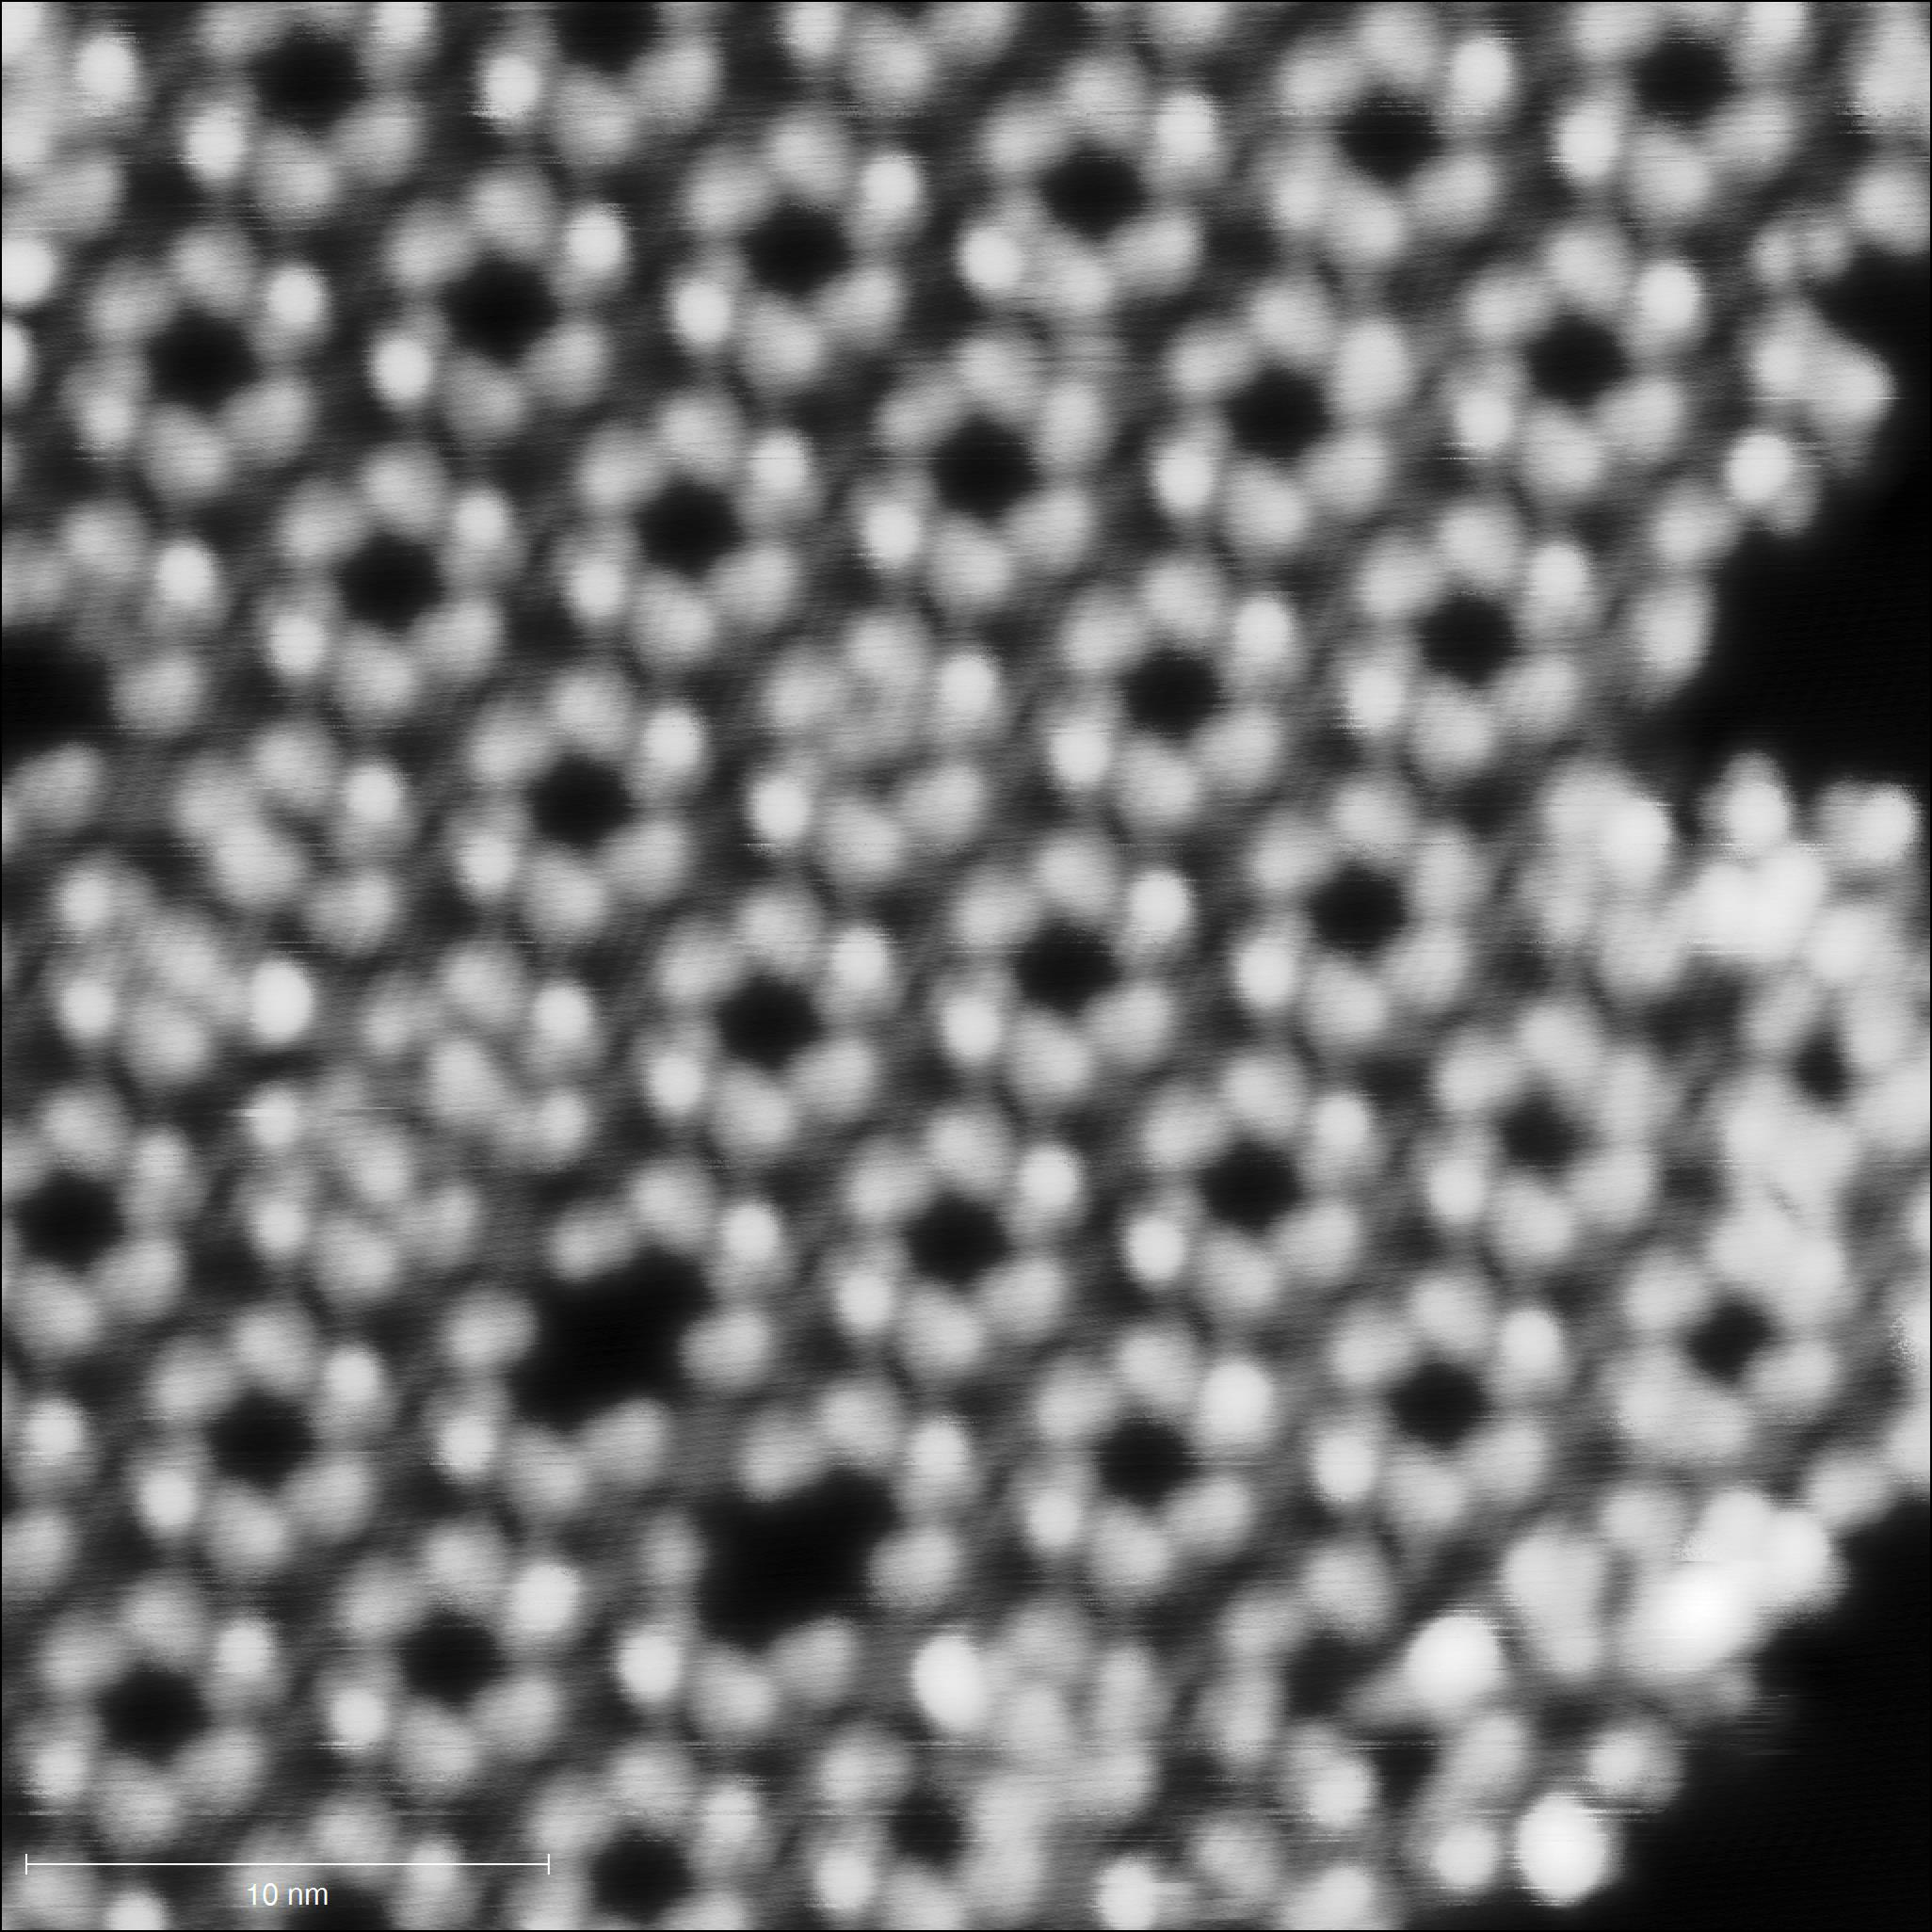
\includegraphics[width=0.45\textwidth]{./images/F160429-185245-R.png}
 }
 \subfigure[Enlarged view on the unit cells]{
 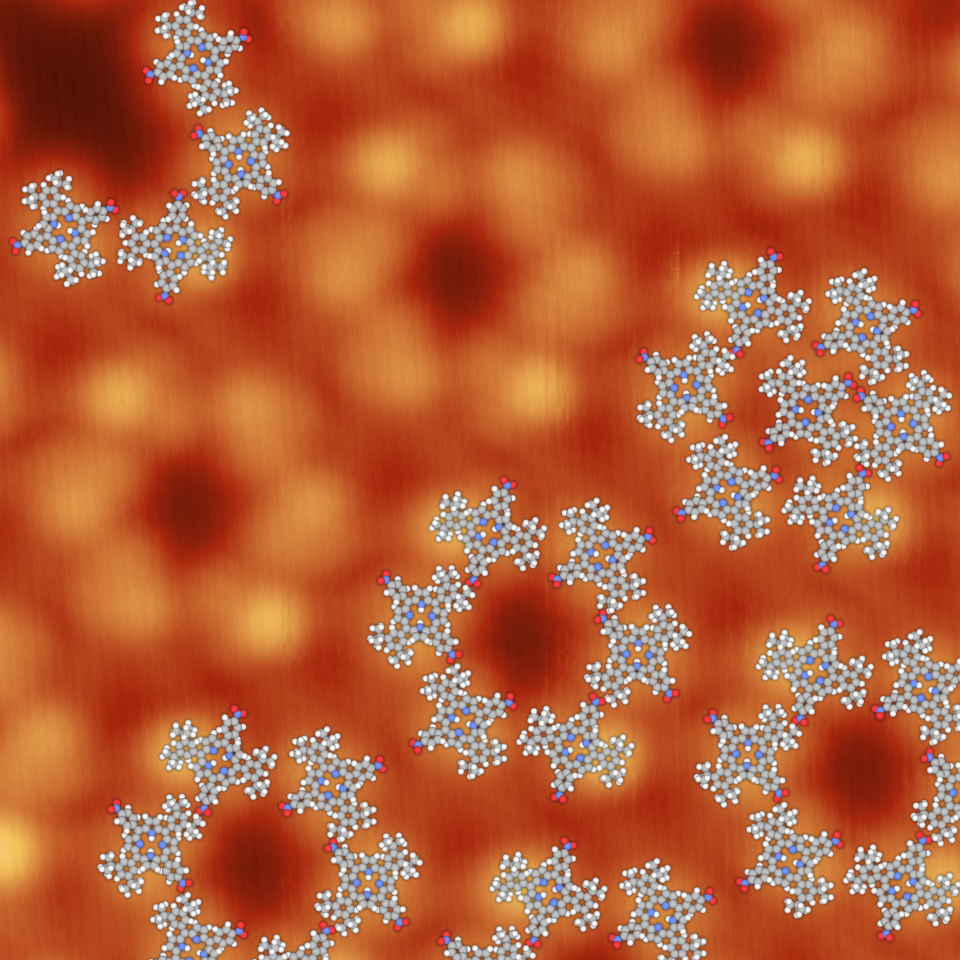
\includegraphics[width=0.45\textwidth]{./images/F160429-185245-R-cut-model.png}
 }
\caption{Trans-TBP adsorped on Ag(100) at room temperature. a) shows a large (37*37nm) fraction of the assembled molecules. The unit cell constituents are enlarged in b) where parts of a) are shown and molecular models overlaid.}
\label{fig:two-leg-trans-ag100-motiv}
\end{figure}